Raft Scope is a visualized developed by the very same protocol author
Diego Ontaro%(@ongardie).
It provides raft basic functionalities simulation, fast forward and run playback;
more precisely it support:
\begin{itemize}
    \item[] \textbf{Protocol}
        \item Leader election
        \item Log replication
    \item[] \textbf{Interaction}
        \item Client request
        \item Server status (start, stop, restart)
        \item Simulation speed
\end{itemize}

\begin{figure}[h]
    \centering
    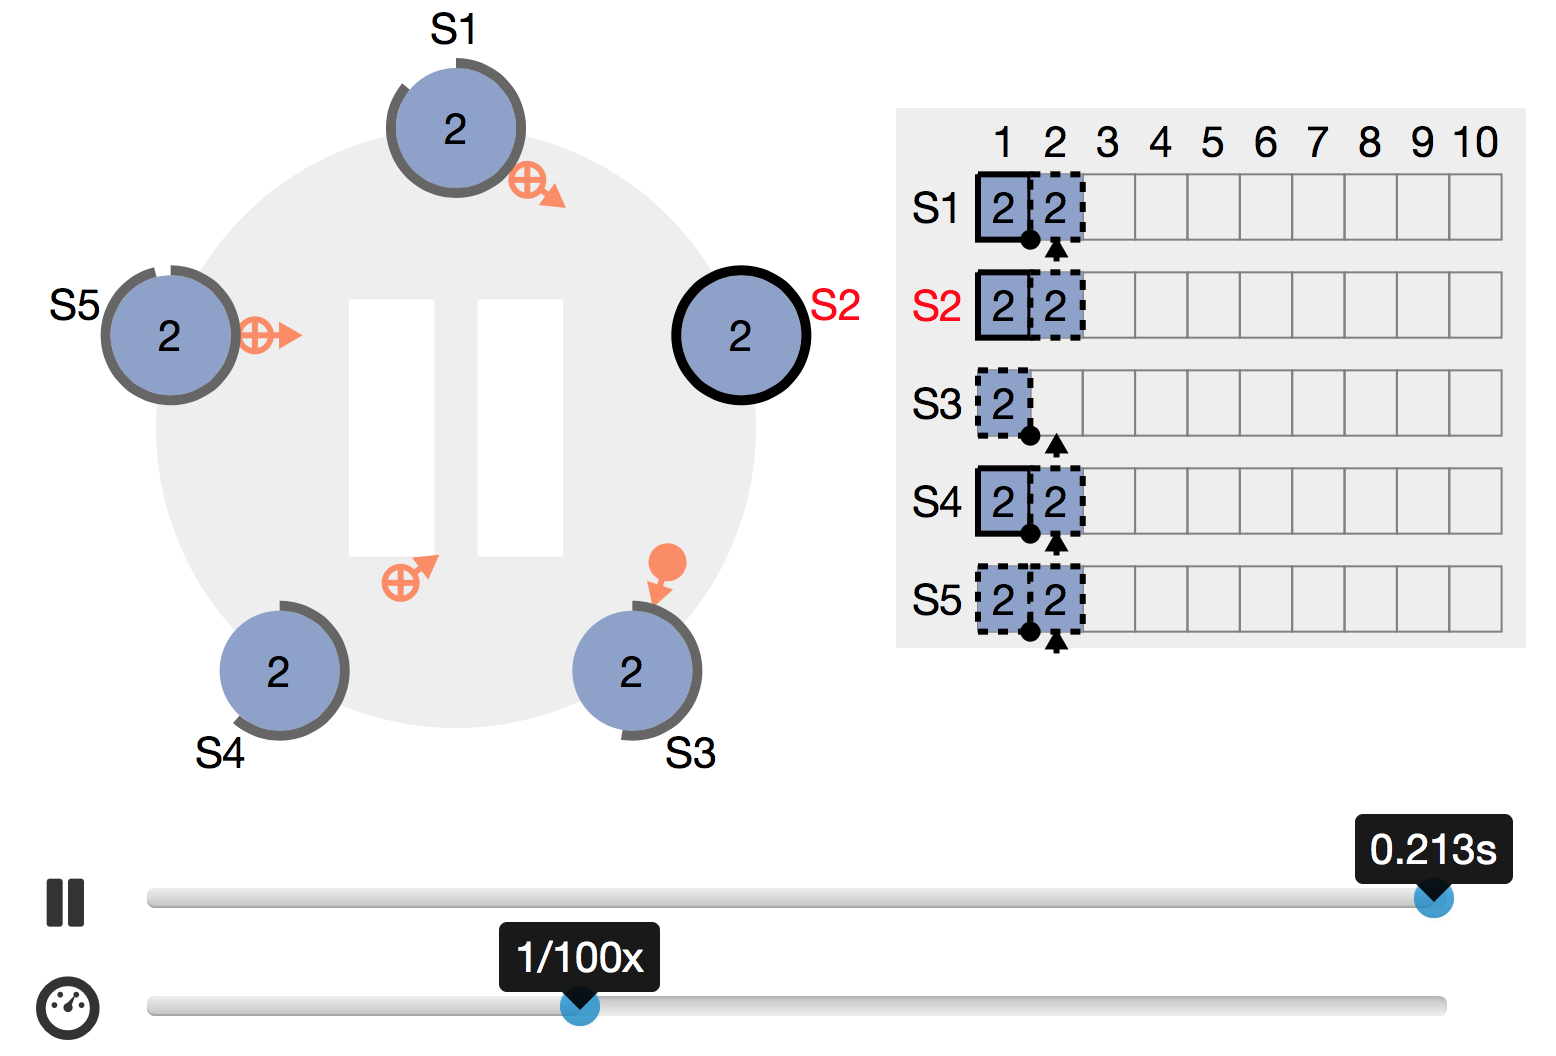
\includegraphics[width=0.9\linewidth]{org.png}
    \caption{Original}\label{fig:original}
\end{figure}

\subsection{Internals}
It is worth nothing that JavaScript it self, language of the simulator,
is single threaded, Ontaro implemented a sort of virtual machine(VM) where the
concurrency is only simulated playing with the concept of time: each action
(\textit{e.g.} receiveMessage) is set to be taken effect at a specific point
in time.
The simulation take place in a main loop (\texttt{raft.update}) where each
server is give the opportunity to make an action(\emph{e.g.} start a new election);
the available action are checked in defined order.
The VM has an internal clock, that at each simulation cycle is
advanced by an amount of time computed \textit{w.r.t} the actual simulation speed.

Due to this design decision many operation are executed in \emph{bulk}, the fact
that they take place in order of due is not worthless but does not guarantee
correctness: Suppose the Leader server~(SL) send an \texttt{AppendEntries} message (M1)
to server 2~(S2), and that the S2 \texttt{ElectionTimeout} is due to expire just after
the M1 arrive, and that the two events take place in the same simulation slice time:
in the real-world S2 would receive M1, reset its \texttt{ElectionTimeout},
and answer with and \texttt{ACK} messager. In the simulation the S2 check for
\emph{start new election} is preformed before the read of the due message,
this lead to S2 actually start a new election.

Fixing this behaviour is not straight forward: swapping the two checks would
break other scenarios (\texttt{e.g.} M1 is due just after the \texttt{ElectionTimeout}).
This without considering what would happen if the simulation speed is in the range
$[ELECTION\_TIMEOUT/2 - ELECTION\_TIMEOUT]$.
The only definitive fix would have been rewriting the entire simulation system.
Given the application of such tool: in-class demonstration/explanation and
visual simulation we preferred to simply limit the speed, to a speed that is
anyhow to fast to understand anything.

Moreover the current design allows to easily take snapshot, action that is
actually performed after each serialization point enabling simulation rewind,
rollback and playback.
